\section{Graph algorithms in \XWS}\label{sec:Graph}

We consider implementations of breadth-first and depth-first search.


\subsection{SIMPLE implementation (C)}

The C implementation of DFS works as follows. First a small stub-tree
of size $O(p^2)$ is generated by one thread randomly walking the graph
starting from the root.  The vertices encountered in the walk are
evenly distributed into the stacks of the $p$ threads. Each thread
then starts traversing the graph in DFS order.  To prevent race
conditions during DFS traversals, lock-free protocols are used to
guard against multiple threads coloring the same vertex. For
load-balancing, a thread attempts to steal a piece of the stack from
another thread in case it runs out of work. As a heuristic, each steal
takes one half of the stack from the victim. Note that in order to
reduce the cost of stealing, no synchronization is invoked in such
steals. The steals may get stale values, yet the correctness is not
jeopardized as the thread will later find all the stolen vertices have
been visited.  When all threads run out of work and there is no work
to steal, the algorithm halt. The stacks and their top and bottom
pointers are declared as volatile, and each push/pop operation
involves operations on volatiles.

The C implementation of parallel BFS follows the SPMD programming
paradigm. The expansion of the BFS frontier is implemented as
follows. Each thread keeps a local queue, and gets an equal portion of
vertices in the current frontier. In the beginning, there is only one
vertex (root) in the frontier, and only one thread has an non-empty
local queue. After draining the current frontier vertices in the
queue, new frontier vertices are placed inside the queue. When all
threads are done with the current frontier (guaranteed with a
barrier), the newly-added vertices in the queues are merged together
to form the new global frontier. Repetitive appearances of nodes in
the frontier is allowed. The algorithm iterates until no new frontier
vertices are discovered.

\subsection{Cilk implementation}

The Cilk implementation of parallel DFS can be derived easily from the
sequential recursive DFS. Instead of sequential traversal, we spawn a
parallel DFS traversal activitiy for each unvisited child of the
current vertex. To guard against race conditions among traversals, the
access to the color of a vertex is protected by lock-free
synchronizations. Load-balancing is handled by the Cilk runtime
library. However, as discussed earlier Cilk forces each procedure to
wait for termination of all activities spawned during its execution.

Computation in Cilk has to be partitioned in a divide-and-conquer way
so as to conform to the Cilk programming model in order to achieve
scalability. To avoid using locks, there are two sets of buffers $Red$
and $Black$ in the Cilk implementation of BFS.  The buffer set $Red$
contains the current BFS frontier, distributed across its member
buffers and initially containing the root vertex. The buffer set
$Black$ will contain the neighbors of the vertices in the current
frontier to form the next one. The Cilk implementation partitions the
current frontier evenly into at most {\tt np} blocks (specified by a
command-line argument). There 
are {\tt np} buffers in each buffer set. The neighbors of
the $i$th block of vertices in the current frontier are stored in
$i$th buffer of the buffer set $Black$. Iteration over the blocks of
the current frontier has to be organized in a divide-and-conquer way
where the base case is the iteration over a single block. Once the
next frontier is formed, the colors of the buffer sets are switched
after a Cilk {\tt sync} statement that functions as a barrier.  As in
the C implementation, repetitive appearances of vertices is
allowed. The algorithm iterates until no new frontier vertices are
discovered.


\subsection{\XWS{} implementation}\label{sec:Performance}

The core code for the \XWS{} implementation is presented in 
Section~\ref{sec:intro}.  We now discuss batching.


%%While classic graph traversals such as DFS and BFS can be supported by
%%XWS, they do not take advantage of some of the algorithm design
%%techniques that exploit work-stealing to provide performance superior
%%to that of other approaches to parallel programming.
%%
%%Work-stealing schemes are natural fits for many classic parallel
%%divide-and-conquer algorithms. (In fact, for some problems and
%%criteria, work-stealing provides optimizal solutions.) For example, to
%%process all of the elements of an array $A$ of size $N$, a root task
%%represents {$A$, $0$, $N$} which is then subdivided into two tasks
%%{$A$, $0$, $n/2$} and {$A$, $n/2$, $n$}, and so on until the size of each
%%task is less than an empirically-guided sequential threshold
%%indicating that further subdivision is not profitable because the task
%%overhead would be greater than the amount of work to process the task
%%sequentially. Notice that in a shared memory environment, the memory
%%needed for task descriptions themselves is small and constant.
%%
Algorithms for irregular graph problems are in general not directly
amenable to divide and conquer recursive decomposition. However, we
can still approximate the properties that make work-stealing perform
well for these problems.

To do this, we first require compact task descriptions.  The size of a
task description representing exploration starting at each of $k$ nodes
should be constant, and independent of $k$. Otherwise, the communication
overhead of pushing and stealing nodes would overwhelm processing,
especially in algorithms such as spanning trees, where the per-node
costs merely amount to marking nodes and labelling their parents.  We
address this by building up lists of work via simple linking: Each
node enqueued in the work-stealing queue is the head of a singly
linked list possibling containing other nodes as well. The ordering of
this list matters only in terms of memory locality and interference
with other threads, which favors simple stack-based linking.

We next ask, what value of $k$ should be used to batch a set of
unprocessed nodes. For any given node in an arbitrary graph, we cannot
know the value that will maximize aggregate throughput.
One choice is to empirically choose some fixed value. However,
the use of any fixed value would be too large during start up
(stalling all but the initial thread), and/or too small during
steady state. We can do better by first characterizing the
best values to use at boundary points:
\begin{itemize}
  \item A queued root node represents all of the work in the graph, so
    requires $k=1$.
  \item If processing has nearly completed, and all remaining nodes are
    dead-ends (i.e., leading to no further expansion) choosing the
    best value of $k$ is the counterpart to choosing the sequential
    threshold of a divide and conquer algorithm.  This value, $S$, is an
    empirical threshold relating algorithmic work versus framework
    overhead.  
\end{itemize}

Unless the per-node costs of an application are high enough to dictate
that $S=1$ (which is not the case for spanning tree algorithms), a rule
that causes $k$ to vary from $1$ at roots to $S$ at collections of dead-ends
will provide better load balance and throughput than would use of a
fixed value. For some special graph types, it is possible to determine
a fixed function of this form. For example, If the graph were actually
a balanced tree, $k$ should increase exponentially from the root to the
leaves. However, in an arbitrary graph, any approach based on distance
from roots would be prone to arbitarily poor estimates.  Intead, each
task may use its current work-stealing queue depth to help estimate
global progress properties: If the queue is empty, then even a single
node placed on it is potentially valuable to some other thread trying
to steal it and further expand.  Conversely, if the queue is very
large, then other threads must be busy processing other nodes, and any
newly discovered node is less likely to lead to further expansion.
Using a simple bounded exponential growth function (here, powers of
two) across these points maintains scaling proprties: Each of the 
$2^j$ nodes in a batch of a size-$j$ queue (for $j \leq log_2(S)$) should have
$2^{-j}$ of the expected expansions as does the single node in a size-$1$
queue. The choice of base two exponents is not entirely forced here,
and different constants might be better for some graph types.
However, the choice does coincide with the scaling and throughput
properties of work-stealing in the case of divide-and-conquer over
balanced binary trees, and adaptively approximates this case by
dynamically varying batch sizes based on differential steal rates.

The resulting basic algorithm is a simple variant of the DFS algorithm
presented in Section~\ref{sec:intro}: Each task accepts a list headed
by one of its nodes.  For each node, it labels and expands the edges
into a new list, pushing that list onto to work-stealing queue when
its size exceeds $min(2^{Q}, S)$, where $Q$ is the queue-size. Notice
that in the case of $S=1$ (which might be used for algorithms with
high per-node processing costs), this is identical to plain DFS.

Our adaptive DFS improves on the implementation of this idea by
incorporating another common work-stealing programming technique. In
classic divide-and-conquer programs, co-execution of two tasks $a$ and $b$
is best implemented by forking $a$, then directly running $b$, and then
joining $a$.  This saves the overhead of pushing and then immediately
popping and running $b$.  We adapt this idea here via some bookkeeping
to swap lists rather than pushing and then immediately popping a new
list when the original list is exhausted. The performance improvements
stemming from this technique are always worthwhile, because they
decrease overhead without changing any other algorithmic
properties. However, as shown below, the extent of the improvement may
vary dramatically across different graph topologies.

As is the case with any work-stealing algorithm, the value of $S$ must
be empirically derived. Thresholds are functions of per-node
application costs (here, marking and setting spanning tree parents),
as well as underlying per-task framework costs (mainly, work-stealing
queue operations), as well as platform-level costs (processor
communication, memory locality effects, garbage collection), along
with interactions among these, and so resist simple analytic
derivation.  However, each of these component factors are properties
of the program, and not, in general, its inputs (i.e., the actual
graphs).  As is the case for all work-stealing algorithms, choosing
values of S larger than necessary will increase the variance of
expected throughput: In some executions this may actually increase
throughput due to less queue overhead, but in others, a too-large
value will cause load imbalances, decreasing throughput.  But
sensitivity curves across these values are shallow within broadly
acceptable ranges. We find that restricting values to powers of two
suffices.

\paragraph{Choice of Threshold}

This choice of threshold was empirically guided by comparing
performance across powers of two. The impact of this choice varies
across graph types. Normalizing to $1.0$ for $S$ of $128$,
Table~\ref{table:rel-perf} shows throughput differences for graphs of
$4$ million nodes.  The best value of $S$ indicates that \XWS{} framework
overhead is low enough that is profitable to parallelize even batches
of only a $100$ or so dead-end nodes. The drop-off beyond $128$ is
very shallow, so larger values could have been used with almost no
loss.  However, choosing thresholds nearer the lower range of
estimated maxima reduces run-to-run variability.

\begin{table}
{\footnotesize
\begin{verbatim}
          Niagara             Opteron
S       Tor  K    Ran     Tor   K     Ran
1      0.58 0.79 0.81    0.18  0.54  0.55
2      0.68 0.85 0.85    0 33  0.78  0.81
8      0.88 0.93 0.94    0.75  0.97  0.93
32     0.97 1.00 0.99    0.82  0.98  0.94
128    1.00 1.00 1.00    1.00  1.00  1.00
512    0.98 0.92 1.00    0.89  1.00  0.99
2048   0.96 0.92 0.91    0.86  0.97  0.97
\end{verbatim}}
\caption{Relative performance across thresholds}\label{table:rel-perf}
\end{table}
While adaptive batching improves performance over DFS (equivalent to
$S=1$) across graph types, the extent of the improvement varies
considerably across graph types. This is due to two main factors,
{\em locality} and {\em connectivity}.

\paragraph{Locality.} The graphs used in these experiments are too large to fit
into processor caches. Thus, cache misses have a huge impact on
performance. The Torus graph is laid out such that each node's
row-wise neighbors will normally be adjacent to it in memory, and
column-wise neighbors a constant stride away. Thus, traversals of a
torus that improve search locality will improve throughput.  This
effect can be quantified by comparing the performance of simply
accessing all of the nodes of the graph via all of its edges in some
predefined locality-sensitive versus locality-insensitive order.  As a
demonstration, the table below shows the relative
improvement of a full scan of each edge of each node when performed in
stride-1 index order of nodes versus a (wrapped around) stride of
$7919$ -- chosen as a prime large enough to minimize cache hits.  

{\footnotesize
\begin{verbatim}
        opteron niagara
Torus   7.4     2.2
K       1.3     1.2
Ran     1.4     1.2
\end{verbatim}}

The
effects on the (4Xdual) Opteron, especially for the Torus graph, are
much larger than on the (single multicore) Niagara. This is due to the
higher relative value of hardware prefetching across processors on the
Opteron when locality prevails.  These results independently indicate
that the ability of adaptive batching to better preserve locality of
access can be either a major or minor source of improvement, depending
on graph layout.  And for torus graphs, spanning tree construction
throughput exceeds that of simple locality-insensitive traversal.

\paragraph{Connectivity.}  For densely or regularly connected graphs, the
ability of a task to swap in a partially created batch when its
initial batch is exhuasted increases the actual nodes processed per
task, up from its nominal value of less than $S$, to the average number
of nodes that may be traversed, with backup partial buffer size of at
most $S$, before hitting a dead end. This value varies signifcantly
across the three graph types we have investigated. For $S=128$, the
average values on the Niagara ranges from $150$ for random graph, to $270$
for k-graphs, to $2400$ for Torus. (Opteron results are similar). As the
numbers of nodes per task increases, so does throughput: Bypassing the
work-stealing queue reduces per-node overhead.  Lower queue access
rates in turn lead to lower contention for threads attempting to steal
work. While these effects are secondary to others described above,
they appear to account for the remaining throughput differences across
graph types.

\subsubsection{Adaptive BFS}

Construction of adaptive BFS in the style of our adaptive DFS
encounters some new obstacles.  BFS proceeds in phases; batching
decisions must apply to next phase, not the current phase. Thus,
decisions cannot rely on current queue state.  Instead we employ a
predictive strategy to control batch sizes. During each phase, each
thread uses its estimate of average workload in the previous phase to
control batch size. Although other choices are possible, we used for
the experiments in Figure~\ref{altair},\ref{moxie}, constant multiples of
the previous estimate, bounded by minimum and maximum sizes. This
requires the multiplier to use as an empirically guided tuning
parameter.

The results demonstrate improvement over non-adaptive versions,
although less extreme than DFS.  We believe that the differences in
magnitude of effects are mainly due to three factors. First, because
BFS requires phased computation, improvements are limited by
underlying barrier synchronization rates (e.g.{} the Opteron's hardware
prefetching does not come into play). Second, our batch size
estimation strategy for BFS cannot be as sensitive to transient
dynamic imbalances as DFS.  And third, the BFS version does not enjoy
as many of the added locality benefits of DFS in-place list-swapping.
As further evidence of this third effect, the best tuning threshold
was higher, and showed sharper sensitivity, on the Opteron MP than the
Niagara multicore, which matches the locality and caching patterns
discussed above.

We leave for future work the investigation of other adaptive rules which may yield better performance. 

\newpage
\onecolumn
\begin{figure}
 \begin{tabular}{ccc}
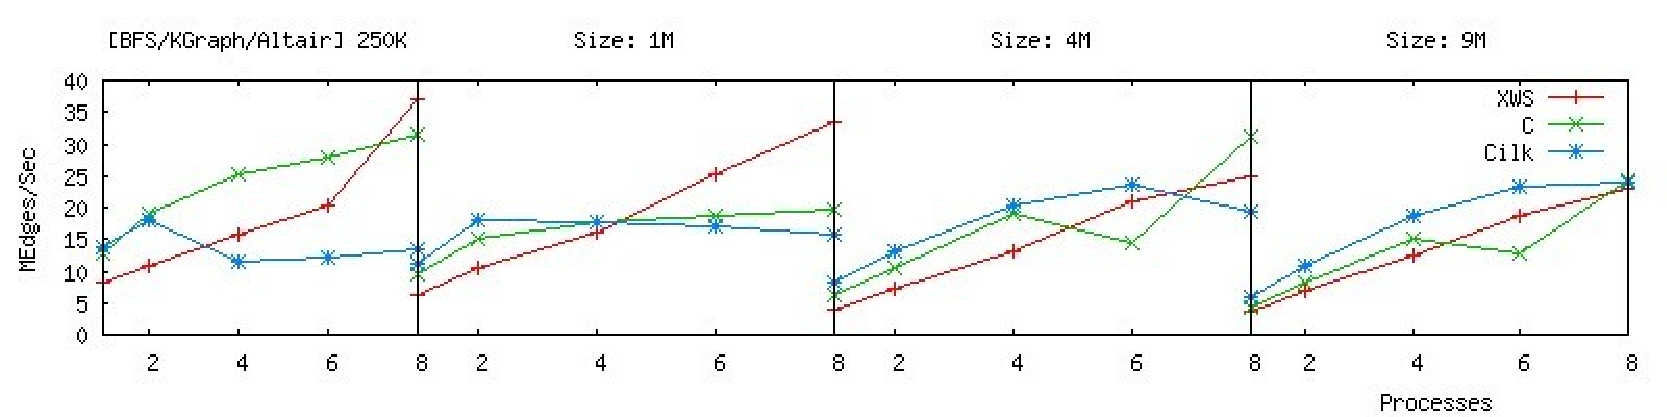
\includegraphics[width=14cm]{../plots/bfs-kgraph-altair-color.pdf} \\
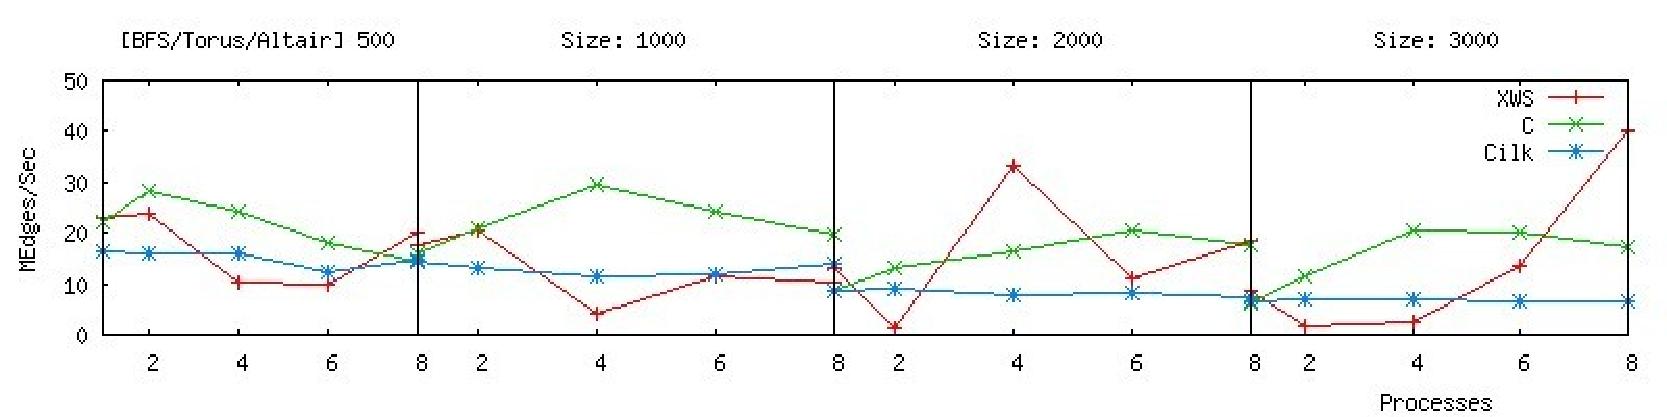
\includegraphics[width=14cm] {../plots/bfs-torus-altair-color.pdf} \\
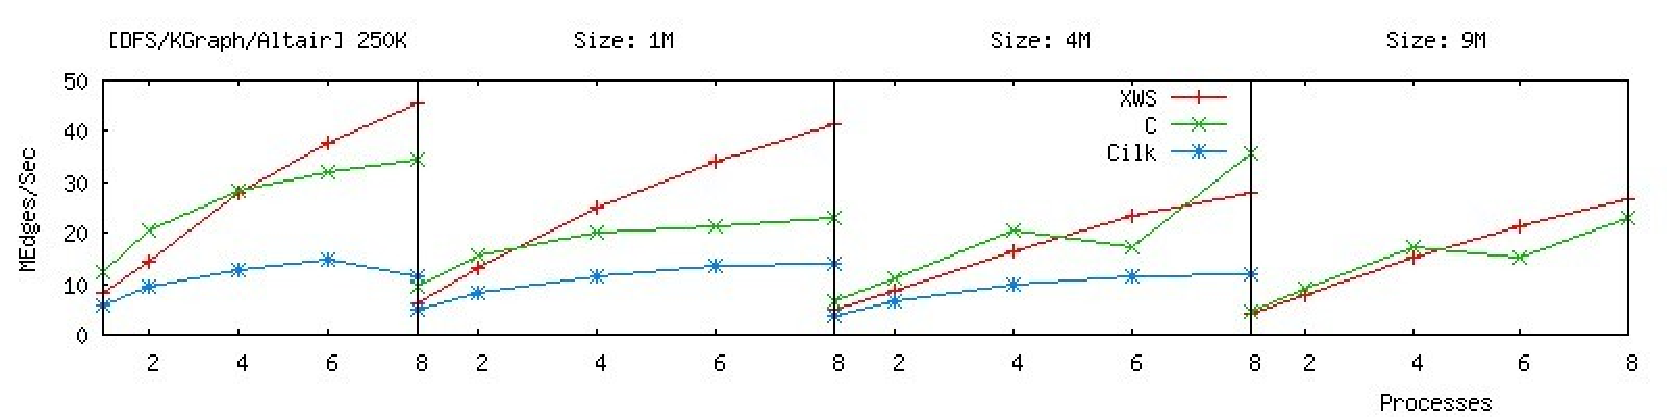
\includegraphics[width=14cm]{../plots/dfs-kgraph-altair-color.pdf}\\
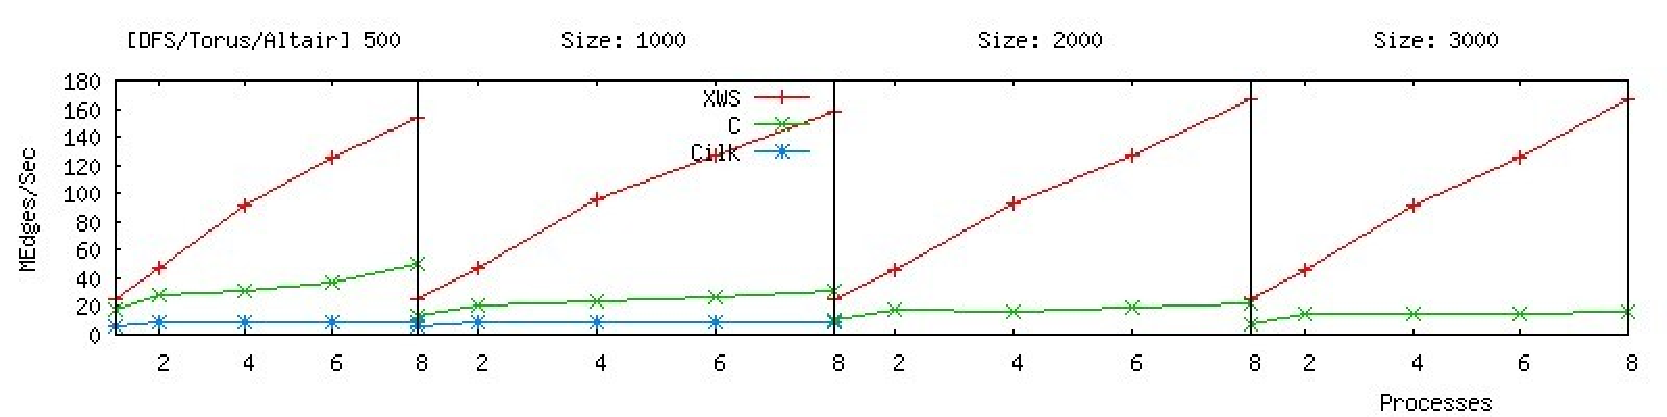
\includegraphics[width=14cm]{../plots/dfs-torus-altair-color.pdf}\\
\end{tabular}
\caption{BFS and DFS for Opteron}\label{altair}
\end{figure}

\begin{figure}
 \begin{tabular}{ccc}
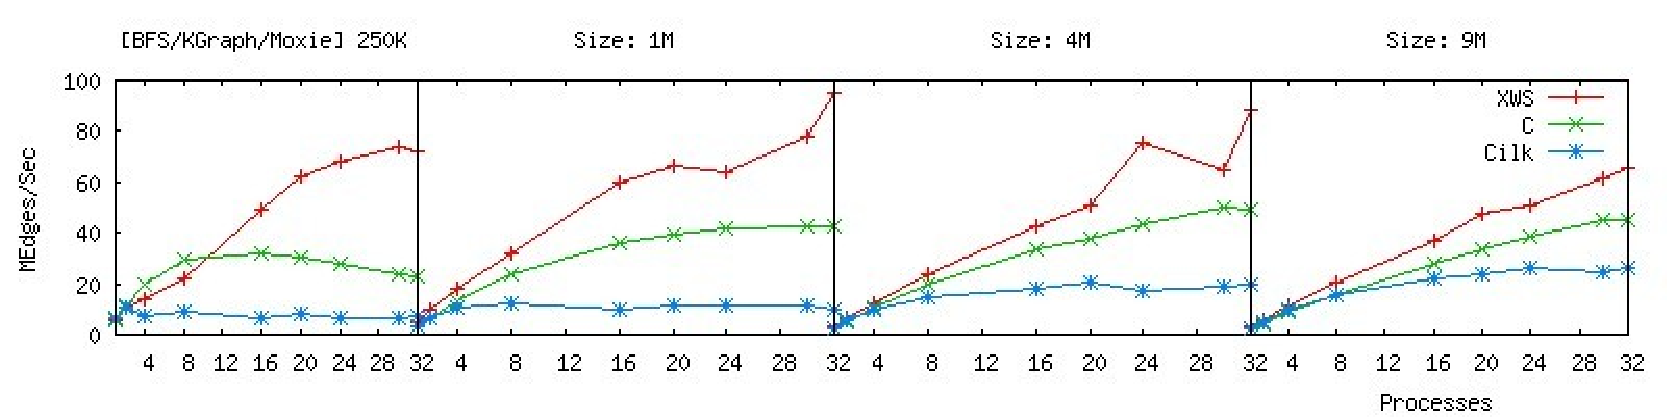
\includegraphics[width=14cm]{../plots/bfs-kgraph-moxie-color.pdf} \\
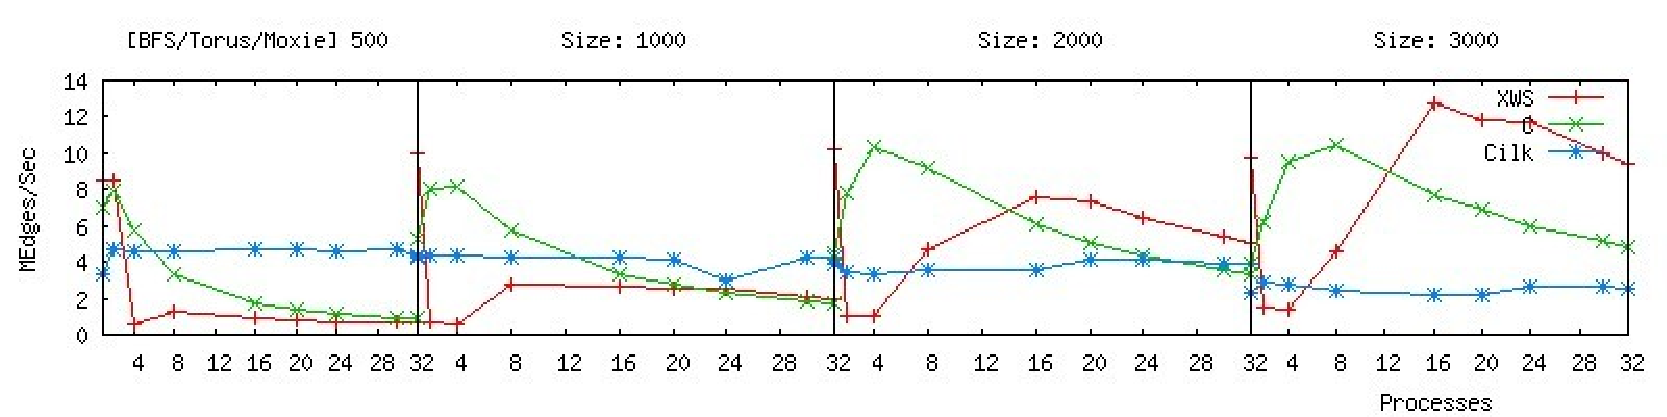
\includegraphics[width=14cm]{../plots/bfs-torus-moxie-color.pdf} \\
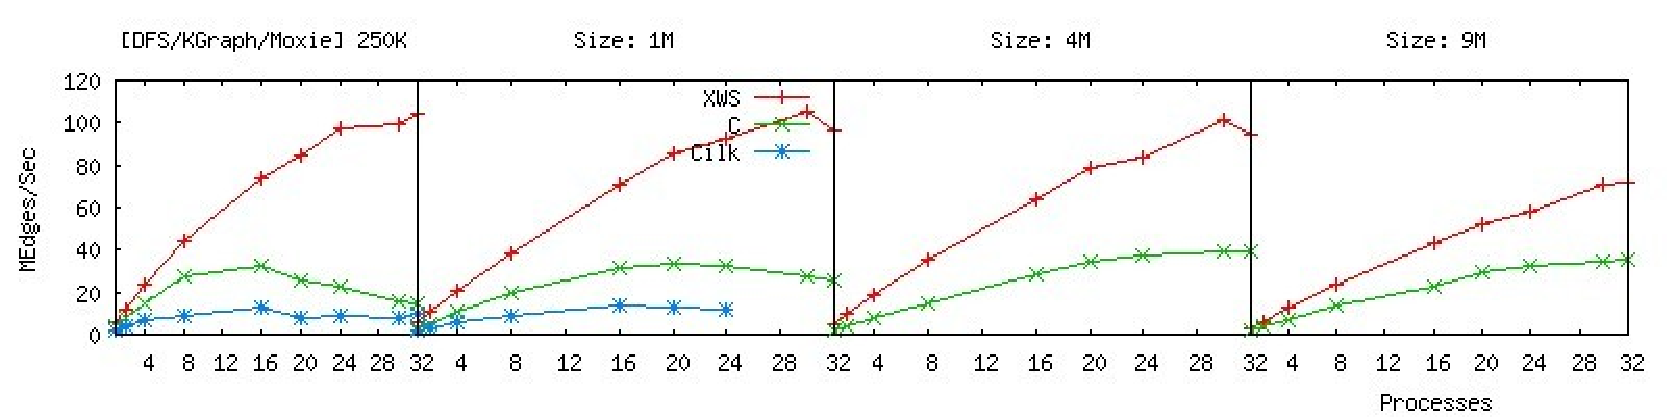
\includegraphics[width=14cm]{../plots/dfs-kgraph-moxie-color.pdf}\\
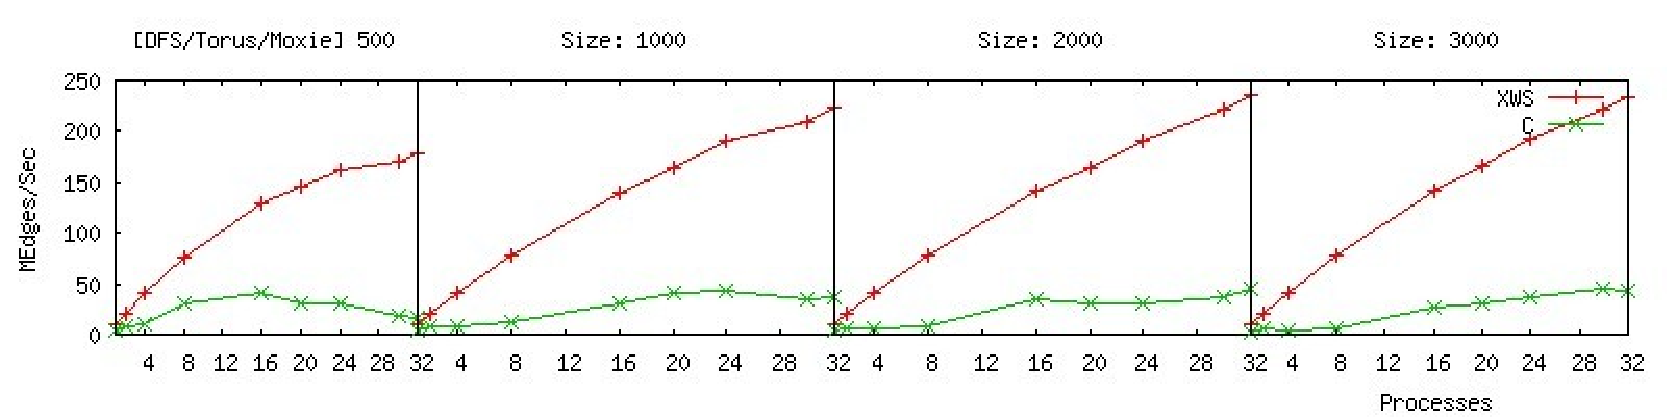
\includegraphics[width=14cm]{../plots/dfs-torus-moxie-color.pdf}\\

 \end{tabular}
\caption{BFS and DFS for Niagara}\label{moxie}
\end{figure}
\twocolumn
\subsection{Results}
We present results in Figure~\ref{altair} for runs of BFS (KGraph,
Random) and DFS (Kgraph, Torus) on Opteron and in Figure~\ref{moxie}
for runs of BFS (KGraph,Torus) and DFS (KGraph, Torus) on Niagara
(y-axis: MEPS, x-axis: P), for 250K, 1M, 4M and 9M vertices.\footnote{
The number of vertices in a torus are the square of the torus
size.}

We see that on Opteron \XWS{} code is comparable with Cilk and C code
for BFS, but substantially outperforms them for DFS. On Niagara,
\XWS{} code substantially outperforms Cilk and C for all three
graphs.\footnote{Several Cilk runs did not complete successfully and
are hence omitted.}

